\hypertarget{_g_r_a_8cpp}{\section{Dokumentacja pliku /home/karolina/\-Pulpit/\-Project41\-Poker(1)/\-Project41\-Poker/\-Project41\-Poker/prj/src/\-G\-R\-A.cpp}
\label{_g_r_a_8cpp}\index{/home/karolina/\-Pulpit/\-Project41\-Poker(1)/\-Project41\-Poker/\-Project41\-Poker/prj/src/\-G\-R\-A.\-cpp@{/home/karolina/\-Pulpit/\-Project41\-Poker(1)/\-Project41\-Poker/\-Project41\-Poker/prj/src/\-G\-R\-A.\-cpp}}
}


Definicja metody klasy \hyperlink{class_g_r_a}{G\-R\-A}.  


{\ttfamily \#include \char`\"{}G\-R\-A.\-h\char`\"{}}\\*
Wykres zależności załączania dla G\-R\-A.\-cpp\-:\nopagebreak
\begin{figure}[H]
\begin{center}
\leavevmode
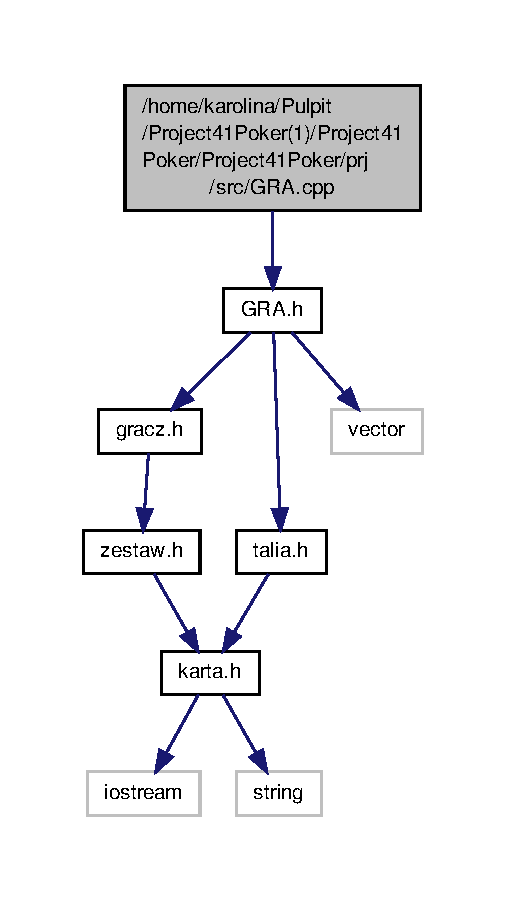
\includegraphics[width=243pt]{_g_r_a_8cpp__incl}
\end{center}
\end{figure}


\subsection{Opis szczegółowy}
Zawiera definicje metod klasy \hyperlink{class_g_r_a}{G\-R\-A}. 

Definicja w pliku \hyperlink{_g_r_a_8cpp_source}{G\-R\-A.\-cpp}.

